\documentclass{article}
\usepackage{amsmath,amsfonts,amssymb,bm,mathtools,upgreek}
\usepackage{caption}
\usepackage{fancyhdr}
\usepackage{float}
\usepackage{fixmath}
\usepackage[T1]{fontenc}
\usepackage[margin=1in]{geometry}
\usepackage{graphicx}
\usepackage{hyperref}
\usepackage[utf8]{inputenc}
\usepackage{lipsum}
\usepackage{siunitx}
\usepackage{subcaption}
\usepackage{optidef}

\graphicspath{ {../figures/} }

\setlength{\parindent}{0pt}
\setlength{\parskip}{.5em}

\title{CS 5033: Final Project Report}
\author{Shane Flandermeyer}
\date{}

% TODO: Make the spacing look good
\begin{document}

\maketitle

\section{Introduction}

The rapid evolution of wireless communications technologies such as 4G/5G and the internet-of-things (IoT)
has radically altered daily life. These technologies utilize the radio frequency (RF) portion of the electro-
magnetic spectrum, which is a finite resource. To effectively access and regulate the spectrum, it is essential
that the next generation of wireless devices be able to rapidly classify and monitor signals in the spectrum.
Information gained from sensing the spectrum can be used for tasks such as cognitive radio, interference
detection, and dynamic spectrum access \cite{Kulin2018}. Signal
detection and classification has traditionally been accomplished through static filtering and
signal processing using expert features \cite{Ariananda2009}. However, a
data-adaptive approach is needed to improve spectrum efficiency to meet modern
wireless data demands.

For this project, I have developed a training and testing dataset generation
tool for RF signal classification networks. This tool follows the process outlined
in \cite{OShea2016}, which uses GNU Radio to simulate the effects of hardware
and propagation through a channel (e.g., free space). The tool is currently
capable of simulating six different types of signals (four
communications-based, two radar-based) and my object-oriented approach makes it
easily extensible to others. To verify the output of the tool, I have also
implemented a modified version of the convolutional neural network (CNN)
described in \cite{OShea2016a}.


\section{Methodology}

For this project, I have implemented a number of radar and communications
signals along with a script to simulate various effects of propagation through a
channel. 
\subsection{Signals}
I will first outline the mathematical definitions of the
various signals (also known as waveforms) I have simulated. The first waveform is
known as binary phase-shift keying (BPSK), which is defined as 

\begin{equation}
    x(t) = \cos(2\pi f_ct + \pi (1-n)), n \in {0,1}
    \label{eq:bpsk}
\end{equation}

BPSK is the most fundamental type of phase modulation used by the communications community. When
the bit to be transmitted is 0, the signal phase is $\pi$, and when the bit is 1
the phase is 0. As equation \ref{eq:bpsk} and figure \ref{fig:bpsk} show,
BPSK is entirely real-valued.

\begin{figure}[H]
    \centering
    \includegraphics[width=0.25\linewidth]{bpsk-const.png}
    \caption{BPSK constellation diagram}
    \label{fig:bpsk}
\end{figure}

I have also implemented higher-order PSK signals: QPSK and 8PSK. QPSK is defined
as

\begin{equation}
    x(t) = \cos(2\pi f_ct + \frac{\pi}{4} (2n-1)), n \in {0,1,2,3}
\end{equation}
 
With this definition, there are four different phase states corresponding to
bits 00, 01, 10, and 11 (figure \ref{fig:qpsk}). Therefore, twice as many bits can be transmitted at
once, and the signal is no longer purely real.

\begin{figure}[H]
    \centering
    \includegraphics[width=0.25\linewidth]{qpsk-const.png}
    \caption{QPSK constellation diagram}
    \label{fig:qpsk}
\end{figure}

8PSK is defined similarly, with eight phase states corresponding to bit
sequences 000, 001, \dots, 111. 

The final communications waveform simulated for this project is known as 16-QAM,
whose constellation diagram is given below

\begin{figure}[H]
    \centering
    \includegraphics[width=0.25\linewidth]{16qam-const.jpg}
    \caption{16-QAM constellation diagram}
    \label{fig:16qam}
\end{figure}

Unlike the previous modulation schemes, the 16-QAM phase states do not lie on
the unit circle. While this allows more bits to be encoded, the phase states
become closer together and are harder to identify in the presence of noise. This
will be important when classification performance is discussed.

To diversify the types of waveforms in the dataset, I have simulated
some radar waveforms as well. The first waveform of this class is known as the
simple pulse or square wave of time duration T, which is defined simply as 

\begin{equation}
    x(t) = \begin{cases}
        1 & \text{if } t \in [0,T] \\
        0 & \text{otherwise}
    \end{cases}
    \label{eq:square}
\end{equation}

The second, known as the linear frequency-modulated (LFM) pulse, is more
complicated and more common in practice

\begin{equation}
    x(t) = \begin{cases}
        \exp\left(j\pi \frac{B}{T}t^2\right) & 0 \leq t \leq T \\
        0 & \text{otherwise}
    \end{cases}
    \label{eq:lfm}
\end{equation}

Here, the waveform frequency sweeps linearly through the bandwidth B over the
pulse duration T. The real and imagninary parts of each
waveform is shown in figure \ref{fig:waveforms}. This representation of the data
serves as the input to the CNN.

\begin{figure}[H]
    \centering
    \includegraphics[width=\linewidth]{waveforms.png}
    \caption{Waveforms used for Experiment}
    \label{fig:waveforms}
\end{figure}

\subsection{Channel Model}
To make the simulated waveforms more representative of real-world scenarios, I
used GNU Radio primitive blocks to implement a channel model. The full mathematical
description of the channel model is

\begin{equation}
    s(t) = \exp(jn_{CFO}(t))\int_{\tau=0}^\infty x(n_{SRO}(\tau)h(t-\tau))d\tau + n_{AWGN}(t)
\end{equation}

Here, $\exp(jn_{CFO}(t))$ is the carrier frequency offset due to free-running
oscillators in the RF hardware. Although the oscillators in the transmitter and
receiver are initially synchronized, they drift apart over time. This
phase/frequency shift was modeled as a random walk process with a Gaussian step
size (with user-defined standard deviation).

The clock timing in each system may also be slightly different, which is
captured in the $n_{SRO}(t)$ term. This is modeled by interpolating the output
signal by a factor of $1 + \beta$, where $\beta$ is the sample rate difference
between systems (normalized by the expected sample rate). For example, if
$\beta = 0.1$, then the receiver collects 11 samples for every 10 samples
transmitted. Ideally, $\beta = 0$.

\begin{figure}[H]
    \centering
    \includegraphics[width=0.5\linewidth]{multipath.png}
    \caption{Example propagation path}
    \label{fig:multipath}
\end{figure}
The model also takes into account the effects of propagation through the
environment, as shown in figure \ref{fig:multipath}.
Ideally, the signal propagates directly from the transmitter to the receiver,
but in practice it will scatter off other objects in the environment to produce
scaled and shifted copies of the original signal. This phenomenon is modeled as
a convolution with an FIR filter $h(t)$, where each filter coefficient
represents an object in the environment. These coefficients also include a
time-varying phase shift to simulate motion and the doppler effect. The final
component of the channel model simulates thermal additive white Gaussian noise
from the receiver. The impact of each of these individual distortions is shown
in figure \ref{fig:channel model} for the reference signal in figure \ref{fig:channel model}(a).

\begin{figure} [H]
    \centering
    \begin{tabular}{cccc}
    \includegraphics[width=0.3\textwidth]{qpsk-rrc.png} &
    \label{fig:qpsk rrc}
    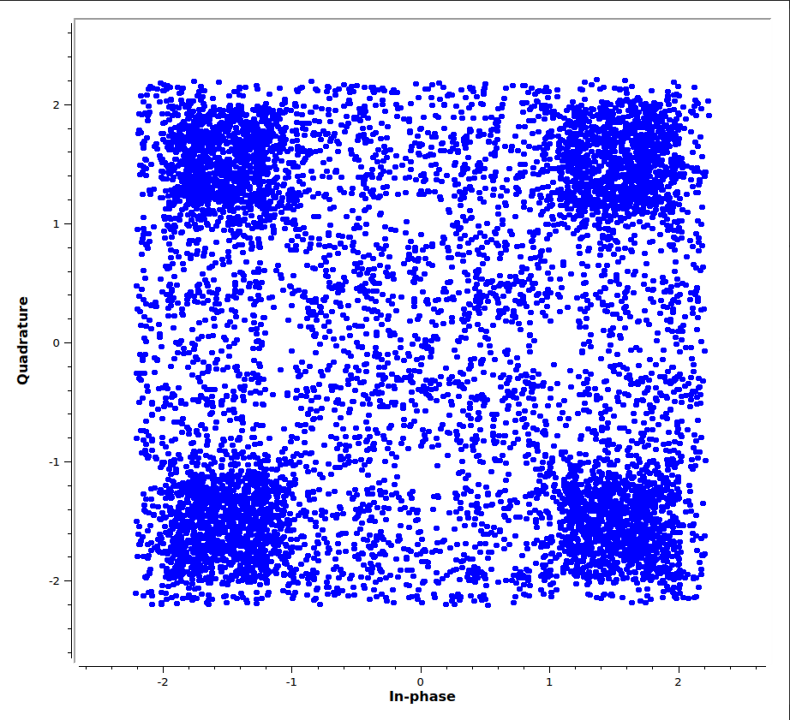
\includegraphics[width=0.3\textwidth]{sro.png} &
    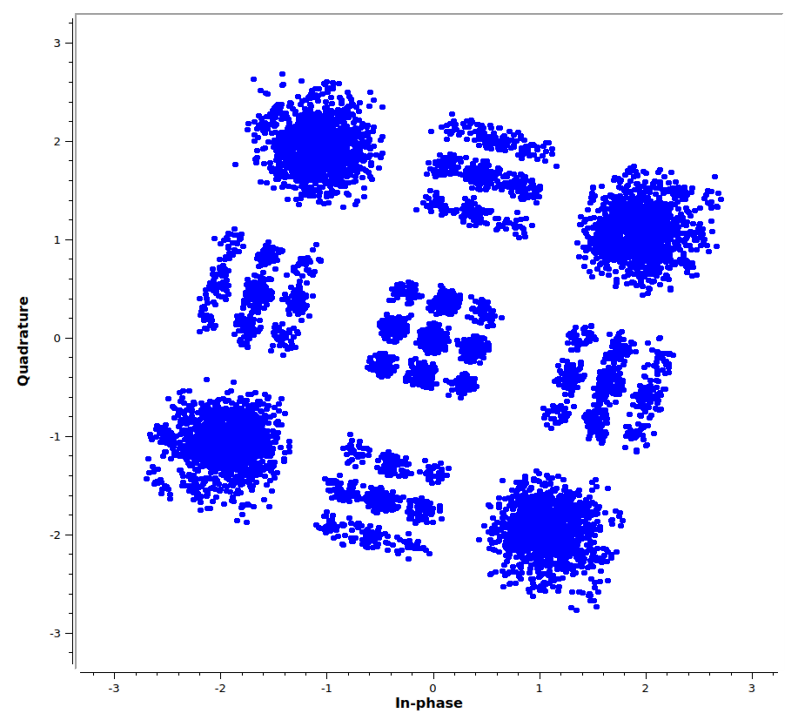
\includegraphics[width=0.3\textwidth]{cfo.png} \\
    \textbf{(a)}  & \textbf{(b)} & \textbf{(c)}  \\[6pt]
    \end{tabular}
    \begin{tabular}{cccc}
    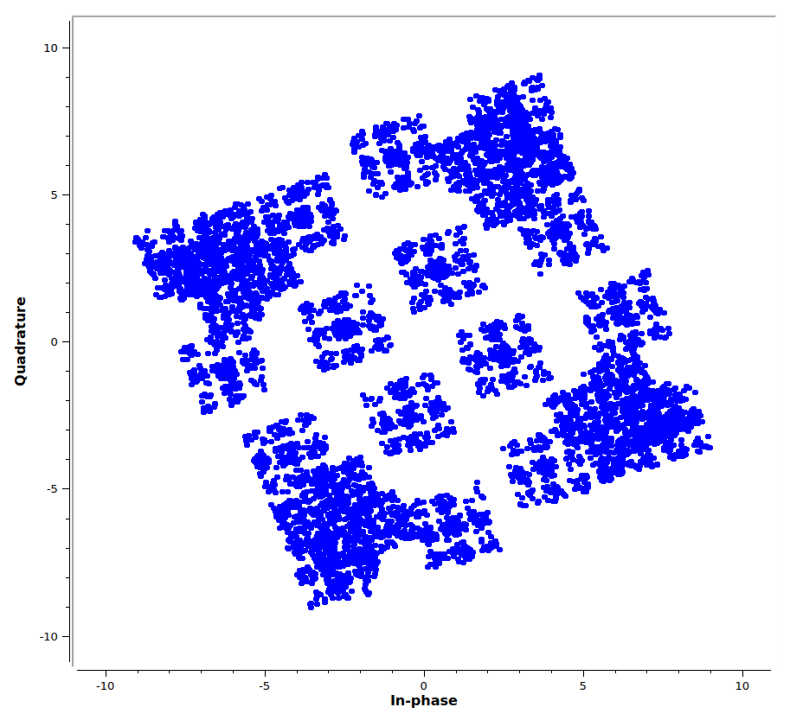
\includegraphics[width=0.3\textwidth]{fading.png} &
    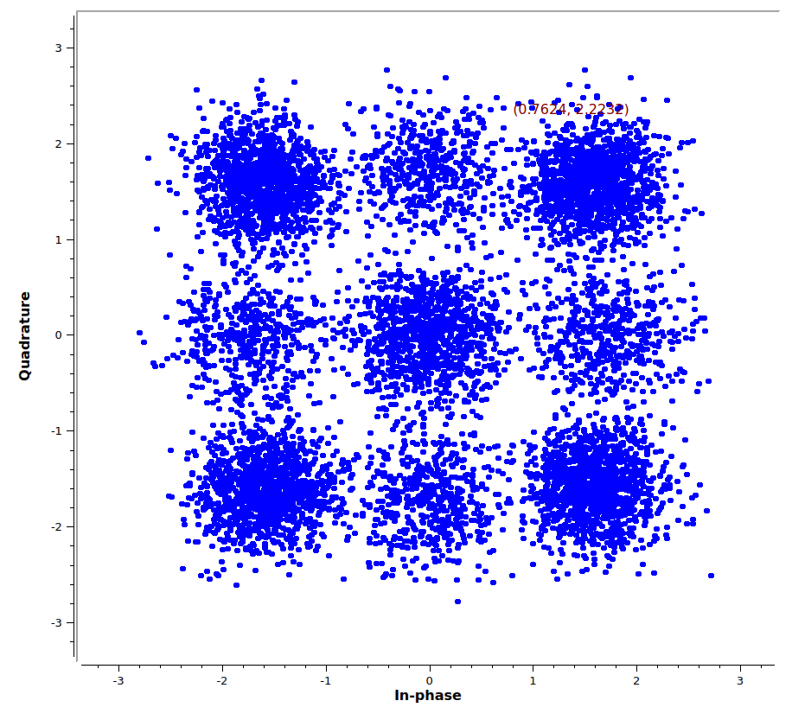
\includegraphics[width=0.3\textwidth]{awgn.png} \\
    \textbf{(d)}  & \textbf{(e)}  \\[6pt]
    \end{tabular}
    \caption{ \textbf{(a)} Root-raised cosine (RRC) filtered QPSK
    \textbf{(b)} Sample rate offset
    \textbf{(c)} Center frequency offset
    \textbf{(d)} Channel fading
    \textbf{(e)} Additive white Gaussian noise}
    \label{fig:channel model}
    \end{figure}

% TODO: Describe the CNN
I also developed a CNN to classify the waveforms using Tensorflow and Keras.
The general architecture given in figure \ref{fig:cnn} is mostly the same as in
\cite{OShea2016a}, but with larger convolution/dense layers and less signals to
classify at the output. Although not shown in the figure, the hidden layers all
use softmax activation functions. Each convolution layer is also preceded by a
zero padding layer to maintain the input size and a dropout layer to mitigate
overfitting. Finally, the Adam optimizer \cite{kingma2017} was used for training.

\begin{figure}[H]
    \centering
    \includegraphics[width=0.5\linewidth]{cnn.png}
    \caption{Classification network architecture}
    \label{fig:cnn}
\end{figure}
\section{Experiment}

\subsection{Data Preparation}
After implementing GNU Radio blocks for the components described above, I used
the GNU Radio streaming architecture to generate the dataset. For each waveform
and noise voltage, I generated 8192 samples of data, then chose a random
length-128 subset of the data to be used as the input to the CNN. For the data
used to generate the figures in this report, I simulated 500 vectors of 10 different noise
voltages for each of the six waveform, resulting in a dataset of size $30000 \times 2
\times 128$. Thus, each training instance was a $2 \times 128$ image, where the
first row is the real part of the signal and the second row is the imaginary
part. These vectors were then normalized to have unit energy, and were
programatically labeled to comply with the SigMF metadata standard \cite{Hillburn2018}.

\subsection{Experiment Design}

Since my simulation tool allows me to generate an arbitrary amount of training data, I
used a 50/50 traning/testing split. There were several channel hyperparameters
to consider such as the magnitude of carrier frequency/sample rate offset, noise
voltage, and channel fading filter parameters. The noise voltage was the
variable I wanted to test, so I varied it over the range -20 dB to 20 dB. The
rest of the channel parameters were chosen to match a ``realistic'' system. For
example, a clock drift of 500 Hz was used because it gives a reasonable mismatch
of 10 parts-per-million for a system operating at a center frequency of 5 GHz.
Since the CNN I built is meant to classify different waveforms, I have chosen to
evaluate performance using classification accuracy.

\subsection{Results and Discussion}
Figure \ref{fig:confusion} gives the model confusion matrix for several
different noise voltages. At high noise voltages (or equivalently, low
signal-to-noise ratios), the model struggles to accurately predict all
waveform classes (figure \ref{fig:noise voltage = 20 dB}) aside from square
waves. This result is intuitive; looking back at figure \ref{fig:waveforms}, it
is easy to see that most waveforms will look similar after noise is added. The
square wave, however, is different enough from the others that it is easy to
classify even with noise. The other extreme is shown in figure \ref{fig:noise
voltage = 0}, where there is still a channel but no noise is present. Here,
classification accuracy is above 80\% for all classes except for 16-QAM and
8PSK, which again makes sense since they look similar even under ideal
conditions. Figure \ref{fig:full test set} gives a more realistic scenario,
where all noise voltage values are present in the training and testing set.
Here, the model still does a poor job of classifying 8PSK and 16-QAM and in
some high-noise situations it had trouble classifying QPSK, but the overall classification
accuracy is about 75\% on average.

\begin{figure}[H]
    \centering
    \begin{subfigure}[b]{0.3\textwidth}
        \centering
        \includegraphics[width=\textwidth]{conf-20dB.png}
        \caption{Noise Voltage = 20 dB}
        \label{fig:noise voltage = 20 dB}
    \end{subfigure}
    \hfill
    \begin{subfigure}[b]{0.3\textwidth}
        \centering
        \includegraphics[width=\textwidth]{conf-infdB.png}
        \caption{Noise Voltage = -$\infty$ dB}
        \label{fig:noise voltage = 0}
    \end{subfigure}
    \hfill
    \begin{subfigure}[b]{0.3\textwidth}
        \centering
        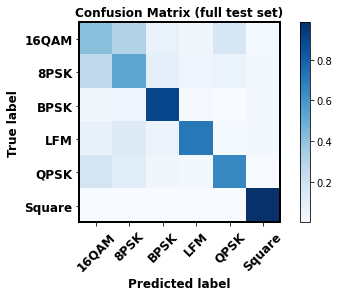
\includegraphics[width=\textwidth]{conf-full.png}
        \caption{Full Test Set}
        \label{fig:full test set}
    \end{subfigure}
       \caption{Confusion Matrices}
       \label{fig:confusion}
\end{figure}

\begin{figure}[H]
    \centering
    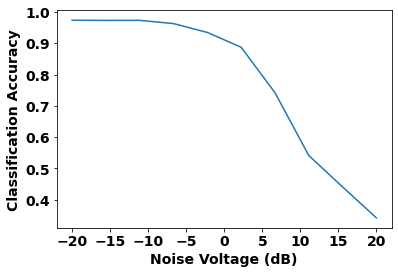
\includegraphics[width=0.45\linewidth]{classification-accuracy.png}
    \caption{Classification Accuracy vs SNR}
    \label{fig:classification accuracy}
\end{figure}

Figure \ref{fig:classification accuracy} more concisely shows the relationship
between classification accuracy and noise voltage. Overall accuracy remains
above 90\% until the noise voltage exceeds around 0 dB, and then it quickly
degrades. Therefore, systems with low-quality (i.e., high noise figure) receiers
would not be able to take full advantage of this classification network, but it
would be quite useful in high-quality hardware.

\bibliographystyle{plain}
\bibliography{../reference} % add reference.bib yourself 

\end{document}
